\chapter{Popis algoritmů}
\section{Kategorie algoritmů}
% přidat definici algoritmu, který řeší mastermind - vytvoří posloupnost kódů, která končí tajným kódem s nejlepším ohodnocením. 
Algoritmy řešící hru Mastermind lze rozdělit do dvou kategorií, \emph{deterministické} a \emph{nedeterministické}. Deterministický algoritmus pro dva shodné stavy volí další krok vždy jednoznačně. 
%Nemůže se tedy stát, že by deterministický algoritmus pro dva stejné vstupy vrátil odlišné výsledky. 
Nedeterministické algoritmy naproti tomu mohou mít v každém stavu na výběr z více následujících kroků. Volit mohou například podle nějakého pravděpodobnostního rozdělení. Není tedy zaručeno, že pro stejný vstup vrátí vždy identický výsledek.

Deterministické algoritmy řešící hru Mastermind mohou mít velikou časovou složitost. To se snaží řešit nedeterministické algoritmy, které hledají rovnováhu mezi časovou složitostí a dobrými výsledky. 
% Hlavní předností deterministických algoritmů je záruka výsledku. Na druhou stranu ale tyto typy algoritmů mohou mít velikou časovou složitost, protože jsou často založeny na procházení všech možností pokračování. To se snaží řešit nedeterministické algoritmy, které hledají rovnováhu mezi časovou složitostí a dobrými výsledky. 
V této práci budeme zkoumat deterministické algoritmy. 

% šlo by zmínit výhody a nevýhody (ne)deterministických algoritmů
% Popsat algoritmy, které hrají pouze kandidáty????

\section{Reprezentace stavu}
% mozna napsat pozdeji ... Všechny deterministické algoritmy, které budeme srovnávat ...


\subsubsection{Orientovaný graf}

% definice inspirovaná matoušek nešetřil
\begin{definice}[Orientovaný graf]
    \emph{Orientovaný graf} definujeme jako dvojici $G = (V,E)$, kde $V$ je množina vrcholů a $E \subseteq V\times V \times Q$ je množina hran s obarveními z množiny $Q$. 
    % Prvky $V$ nazýváme vrcholy a prvky $E$ hrany. 
    Řekneme, že z vrcholu $A \in V$ do vrcholu $B \in V$ vede hrana obarvená $q \in Q$, pokud $(A,B,q) \in E$. Navíc $E$ je taková, že z libovolného vrcholu nevedou dvě různé hrany se stejným obarvením.
\end{definice}
\begin{pozn}
    Orientovaný graf povoluje více hran mezi stejnými vrcholy, které se ale liší v obarvení. Hrana je navíc jednoznačně určena počátečním vrcholem a obarvením.
\end{pozn}

\begin{definice}[Cesty v grafu]
    Nechť $G = (V, E)$ je orientovaný graf s množinou obarvení hran $Q$.
    \emph{Orientovaná cesta} je konečná (i prázdná) posloupnost navazujících hran (ve vrcholech).
    % z vrcholu $A \in V$} definujeme jako konečnou posloupnost navazujících hran začínající ve vrcholu $A$. 
    % Řekneme, že do vrcholu $B$ vede z vrcholu $A$ orientovaná cesta $P = (E_1, \dots, E_m)$, pokud $A$ je první vrchol $E_1$ a $B$ je druhý vrchol $E_m$. 
    % Značíme ji posloupností obarvení hran.
    % $P = ((u_1,r_1), \dots, (u_j, r_j))$. 
    \emph{Neorientovaná cesta} je konečná posloupnost navazujících prvků $(C,D,q) \in V \times V \times Q$ taková, že pro každý prvek posloupnosti platí, že $(C,D,q) \in E$ nebo $(D,C,q) \in E$. 
    % z vrcholů $E_m$ a druhá a předposlední hrana navazují na první a poslední hranu ve odlišném vrcholu než $A$ respektive $B$.
    % hran $P = (E_1, \dots, E_m) , \hspace{3px} E_i\in E$ taková, že $E_i, E_{i+1}$ mají společný vrchol pro $i = 1,\dots,m-1$. Řekneme, že neorientovaná hrana $P$ vede mezi vrcholy $A$ a $B$, pokud $A$ je jeden z vrcholů $E_1$ a $B$ je jeden z vrcholů $E_m$.
    % Řekneme, že orientovaný graf $G=(V,E)$ je souvislý, pokud mezi libovolnými vrcholy $A, B \in V$ existuje posloupnost navazujících prvků $(C,D) \in V \times V$, taková, že pro každý prvek posloupnosti platí, že $(C,D) \in E$ nebo $(D,C) \in E$.  
    Řekneme, že cesta $P = (E_1, \dots, E_m)$
    % , \hspace{3px} E_i\in E$
    je \emph{konstantní}, pokud existuje vrchol $A \in V$ takový, že pro $i = 1,\dots,m $ platí, že $E_i = (A,A,q)$ pro nějaké $q \in Q$. 
    \emph{Redukovaná cesta} je cesta, ve které se každý prvek vyskytuje nejvýše jednou. V případě redukované neorientované cesty nepovolujeme dva prvky, které se liší pouze obrácením vrcholů.
    % Konstantní posloupnost vede do počátečního vrcholu. 
    % Řekneme, že do vrcholu $K_2$ vede cesta z vrcholu $K_1$, pokud se z vrcholu $K_1$ dostaneme do vrcholu

    Řekneme, že cesta $P = (E_1, \dots, E_m)$ vede mezi vrcholy $A$ a $B$, pokud $A$ je první vrchol $E_1$ a $B$ je druhý vrchol $E_m$. 
\end{definice}
\begin{pozn}
    Cesta je jednoznačně určena počátečním vrcholem a obarvením hran, protože z libovolného vrcholu vede s nějakým obarvením maximálně jedna hrana. Prázdná posloupnost je také cesta a je konstantní. 
    % Neorientovaná cesta je to, co si člověk pod ní automaticky představí. 
\end{pozn}
\begin{pozn}\label{pozn-redukce-cesty}
    Z libovolné uzavřené cesty $P$ z vrcholu $A$ vytvoříme redukovanou tak, že vezmeme první vrchol $C$ v cestě $P$ (kromě $A$), který se v této cestě vyskytuje dvakrát. Odstraněním všech hran mezi hranami s prvním a posledním výskytem vrcholu $C$ dostaneme uzavřenou redukovanou cestu z vrcholu $A$.
\end{pozn}
% \begin{lemma}
%     Nechť existuje cesta z vrcholu 
% \end{lemma}
% \begin{dukaz}
    
% \end{dukaz}


\begin{definice}[Souvislý graf]
    Řekneme, že orientovaný graf $G=(V,E)$ je \emph{souvislý}, pokud mezi libovolnými vrcholy $A, B \in V$ existuje neorientovaná cesta.
\end{definice}

\begin{definice}[Kořen a list]
    Nechť $G = (V, E)$ je orientovaný graf. \emph{Kořen} je vrchol, do kterého nevede žádná hrana. \emph{List} je vrchol, ze kterého nevede žádná hrana.
\end{definice}

\begin{definice}[Cyklus]
    \emph{Neorientovaný cyklus} nezveme uzavřenou redukovanou neorientovanou cestu kladné délky.
    \emph{Orientovaný cyklus} nazveme uzavřenou redukovanou orientovanou cestu kladné délky.
\end{definice}

\begin{definice}[Strom]
    Řekneme, že orientovaný graf $G=(V,E)$ je \emph{strom}, pokud je souvislý a neobsahuje neorientovaný cyklus. Řekneme, že strom je \emph{kořenový}, pokud má právě jeden kořen a do každého vrcholu z něj vede orientovaná cesta. 
\end{definice}
\begin{pozn}
    Strom nemusí obsahovat kořen, pokud je jeho množina vrcholů nekonečná. 
\end{pozn}

\begin{lemma}\label{lemma-char-korenoveho-stromu}
    Nechť $G=(V,E)$ je souvislý orientovaný graf s jedním kořenem takový, že do každého vrcholu $A \in V$ vede orientovaná cesta z kořene. Potom $G$ je kořenový strom právě tehdy, když do každého vrcholu $A \in V$ vede maximálně jedna hrana. 
\end{lemma}
\begin{dukaz}
    Nechť napřed $G$ je kořenový strom a nechť existuje vrchol $A$ v kořenovém stromu, do kterého vedou dvě hrany, $E_1$ a $E_2$. Potom tyto hrany vedou z odlišných vrcholů, protože jinak bychom dostali neorientovaný cyklus mezi dvěma vrcholy. Označíme je $B_1$ a $B_2$. Do obou vrcholů vede z definice orientovaná cesta z kořene. Tyto cesty označíme $P_1$ a $P_2$. Potom existuje neorientovaná uzavřená cesta z vrcholu $A$ ve tvaru $P = E_1^*, P_1^*, P_2, E_2$. Operace $^*$ obrátí pořadí vrcholů v cestě a prohodí oba vrcholy ve všech hranách. Z této cesty vytvoříme redukovanou podle poznámky \ref{pozn-redukce-cesty}. 
    % tak, že vezmeme první vrchol $C$ v cestě $P$ (kromě $A$), který se v této cestě vyskytuje dvakrát. Odstraněním všech hran mezi hranami s prvním a posledním výskytem vrcholu $A$ dostaneme neorientovaný cyklus z vrcholu $A$. 
    Tak dostaneme neorientovaný cyklus, což je ve sporu s neexistencí neorientovaných cyklů ve stromu.
    % a tedy z každého vrcholu kořenového stromu vede nejvýše jedna hrana.

    Druhou implikaci dokážeme sporem. Nechť $G$ není strom. Potom existuje nějaký neorientovaný cyklus $P = E_1, \dots , E_m$ z vrcholu $A \in V$. Nad hrany nadepíšeme šipky. Pokud $E_i \in E$, nakreslíme nad $E_i$ šipku doprava. Pokud $E_i \notin E$, nakreslíme nad hranu šipku doleva. Tyto šipky ukazují směr hran v grafu $G$ mezi vrcholy ve kterých se v průběhu cesty \uv{nacházíme}. Pokud $\overrightarrow{E_1}, \dots , \overleftarrow{E_m}$, tak v cestě existuje vrchol, do kterého vedou dvě hrany. Pokud $\overleftarrow{E_1}, \dots , \overrightarrow{E_m}$, tak do vrcholu $A$ vstupují dvě hrany. Nechť $\overrightarrow{E_1}, \dots , \overrightarrow{E_m}$ (obdobně opačný směr). Předpokládejme, že se směr šipek uvnitř cesty nezmění (jinak by existoval vrchol, do kterého vedou dvě hrany). Víme, že existuje cesta z kořene do vrcholu $A$. Cyklus $P$ nevede přes kořen, protože do kořene nevede žádná hrana. Tedy existuje nějaký vrchol $B \in V$, přes který vede cyklus $P$, a do kterého navíc vede hrana na cestě z kořene do vrcholu $A$. Tedy existuje vrchol, do kterého vedou dvě hrany, což je spor. 
\end{dukaz}

Definujeme podgraf inspirovaný definicí z (Matoušek, Nešetřil, \cite{matouvsek2009kapitoly}, str. 101).
\begin{definice}[Podgraf]
    Nechť $G = (V,E)$ a $G_2 = (V_2, E_2)$ jsou orientované grafy se stejnou množinou obarvení hran $Q$ a $V_2 \subseteq V$. Řekneme, že $G_2$ je \emph{podgraf grafu $G$}, pokud $E_2 \subseteq V_2 \times V_2 \times Q$ a zároveň $E_2 \subseteq E$.
    Řekneme, že $G_2$ je \emph{podgraf grafu $G$ indukovaný množinou $V_2$}, pokud $E_2 =  E \cap V_2\times V_2 \times Q$.
\end{definice}

% \begin{lemma}\label{lemma-max-jedna-vchazejici-cesta}
%     Do každého vrcholu v kořenovém stromu vede nejvýše jedna hrana.
% \end{lemma}
% \begin{dukaz}
%     Nechť existuje vrchol $A$ v kořenovém stromu, do kterého vedou dvě hrany, $E_1, E_2$. Potom tyto hrany vedou z odlišných vrcholů, protože jinak bychom dostali neorientovaný cyklus mezi dvěma vrcholy. Označíme je $B_1$ a $B_2$. Do obou vrcholů vede z definice orientovaná cesta z kořene. Tyto cesty označíme $P_1$ a $P_2$. Potom existuje neorientovaná uzavřená cesta z vrcholu $A$ ve tvaru $P = E_1, P_1^*, P_2, E_2$, kde $P_1^*$ je cesta $P_1$ s obráceným pořadím hran. Z této cesty vytvoříme redukovanou tak, že vezmeme první vrchol $C$ v cestě $P$ (kromě $A$), který se v této cestě vyskytuje dvakrát. Odstraněním všech hran mezi hranami s prvním a posledním výskytem vrcholu $A$ dostaneme neorientovaný cyklus z vrcholu $A$. To je spor s neexistencí neorientovaných cyklů ve stromu, a tedy z každého vrcholu kořenového stromu vede nejvýše jedna hrana.
% \end{dukaz}

\begin{tvrz}\label{tvrzeni-podgraf-korenoveho-stromu}
    Neprázdný souvislý podgraf kořenového stromu je kořenový strom.
\end{tvrz}
\begin{dukaz}
    Označíme $G$ kořenový strom a $T = (V,E)$ jeho neprázdný souvislý podgraf. Potom $T$ je jistě strom, protože pokud by obsahoval uzavřenou redukovanou neorientovanou cestu kladné délky, tato cesta by byla i v původním grafu $G$. 

    Pokud by podgraf $T$ neobsahoval kořen, existovala by nekonečná posloupnost vrcholů v $T$, $A_1, A_2, \dots$ propojená hranami z $A_i$ do $A_{i-1}$. Do všech vrcholů $A_i$ ale v grafu $G$ vede nějaká orientovaná cesta z kořene. Navíc do každého vrcholu v kořenovém stromu vede maximálně jedna hrana díky lemmatu \ref{lemma-char-korenoveho-stromu}. Tedy platí, že cesta z kořene původního stromu do $A_1$ vede přes $A_i$ pro všechna $i \in \mathbb{N}$. To je ale spor s konečností cesty. 

    Podgraf $T$ tedy obsahuje nějaký kořen. Pokud by obsahoval dva kořeny, pak mezi nimi díky souvislosti vede neorientovaná cesta. Tuto cestu lze redukovat obdobně jako v poznámce \ref{pozn-redukce-cesty}. Protože do kořene nevede hrana, první a poslední hrana této cesty vede z kořene ven. Když se z obou stran cesty budeme blížit do středu, všechny hrany vedou směrem od kořenů díky redukovanosti cesty a lemmatu \ref{lemma-char-korenoveho-stromu}. Na této cestě tedy musí existovat nějaký vrchol, do kterého vedou dvě různé hrany, což je spor. Toto pozorování je obdobné konstrukcím šipek nad hranami v důkazu lemmatu \ref{lemma-char-korenoveho-stromu}. Podgraf $T$ tedy obsahuje jediný kořen.
    
    Díky souvislosti do každého vrcholu z $T$ vede neorientovaná cesta. Zároveň redukovaná verze této cesty bude orientovaná, protože ve chvíli, kdy se do nějakého vrcholu dostaneme po správném směru hrany, tak všechny dosud \uv{neprozkoumané} hrany vedou z vrcholu ven. Navíc z kořene vedou všechny hrany ven. Tedy $T$ je kořenový strom a pro každý vrchol existuje právě jedna orientovaná cesta z kořene vedoucí do tohoto vrcholu po jediné \uv{vcházející} hraně.
\end{dukaz}

%%%%%%%%%%%%%%%%%%%%%%%%%%%%%%%%%%%%%%%%%%%%%%%%%%%%%%%%%%%%%%%%%

\subsubsection{Stav hry}
V každém kroku algoritmů vycházíme z určitého stavu hry, pro který daná metoda vybírá další pokus. Stav je posloupnost pokusů s ohodnocením a jsou to přesně ty informace, které má hráč [n,k]-Mastermindu k dispozici, a na základě kterých volí následující tah.

\begin{definice}[Kolo a stav]\label{stav}
   \emph{Kolo} definujeme jako dvojici $(u,r)$, kde $u \in H_{n,k}$ je kód a $r \in S_{n,k}$ je ohodnocení. 
   % Nechť $j \in \mathbb{N}$, $u_1, \dots , u_j \in H_{n,k}$ jsou kódy a $r_1, \dots, r_j \in S_{n,k}$ ohodnocení. 
   \emph{Stav} definujeme jako konečnou posloupnost kol $((u_1, r_1), \dots, (u_m, r_m))$. \emph{Počáteční stav} definujeme jako prázdnou posloupnost $()$.
\end{definice}
% Vazby stavů budeme interpretovat jako v kořenovém stromu, kde vrcholy odpovídají stavům. Hrany znázorňují pokusy s ohodnocením, které [n,k]-Mastermind posouvají do dalších stavů. 

Stavy hry a vazby mezi nimi popíšeme orientovaným grafem. Hrany znázorňují pokusy s ohodnocením, které hru [n,k]-Mastermind posouvají do dalších stavů. 
\begin{definice}[Strom \text{[n,k]-Mastermindu}]
  \emph{Strom [n,k]-Mastermindu} definujeme jako orientovaný graf na množině všech stavů. Ze stavu $A = \left((u_1, r_1),\dots, (u_j,r_j)\right)$ do stavu $B = \left((w_1, s_1), \dots, (w_l,s_l)\right)$ vede hrana právě tehdy, když $l = j+1$ a pro všechna $ i \in \{1,2,\dots, j\}$ platí $ (u_i, r_i) = (w_i, s_i)$. Tato hrana je obarvená kolem $(w_l, s_l)$, tedy kódem $w_l$ a ohodnocením $s_l$.
  % Z počátečního stavu vede hrana do všech stavů $(u,r)$ pro $u \in H_{n,k}$ a $r\in S_{n,k}$.
\end{definice}
\begin{pozn}
    Strom [n,k]-Mastermindu má nekonečnou množinu vrcholů. Každý vrchol je ale konečným stavem.
\end{pozn}
\begin{pozorovani}
    Strom [n,k]-Mastermindu je kořenový strom.
\end{pozorovani}
\begin{dukaz}
    Do všech stavů kromě počátečního vede právě jedna hrana z vrcholu, který vznikne vynecháním posledního kola stavu. Tedy počáteční stav je jediným kořenem. Navíc do všech stavů $A$ vede orientovaná cesta z počátečního stavu daná koly ve stavu $A$, kde kolo slouží jako obarvení hrany. Pozorování plyne z lemmatu \ref{lemma-char-korenoveho-stromu}.

    % Stačí tedy dokázat neexistenci neorientovaného cyklu.
    %  Uvažujme stav $A$, ze kterého vede neorientovaný cyklus. Uvažujeme první a poslední hranu. Nechť jsou tyto hrany mezi stavem $A$ a jeho následníky, například $A_{u,r}, A_{v,t}$, $(u,r) \neq (v,t)$. Potom díky redukovanosti cyklu jsou všechny vrcholy cesty prodloužením buď $A_{u,r}$ nebo $A_{v,t}$. Hrana mezi těmito prodlouženími nemůže existovat, protože se stavy liší hned u následníka stavu $A$.

    % Obdobně pokud jedna krajní hrana cyklu spojuje stav $A$ se stavem $B$, ze kterého vede do stavu $A$ hrana, tak 
    
    % potom neexistuje hrana mezi libovolným prodloužením stavu $A_{u,r}$ a libovolným prodloužením stavu $A_{v,t}$, protože se liší hned u následníka stavu $A$. Zároveň neexistuje hrana mezi libovolným
\end{dukaz}

Stavy, do kterých ze stavu $A$ vede nějaká hrana nazýváme následníky stavu $A$. 
%Zavádíme definici potomka množiny, která s potomkem stavu přímo souvisí. 

\begin{definice}[Následník stavu]\label{potomek}
  % Uvažujme [n,k]-Mastermind s nějakým tajným kódem $v\in H_{n,k}$. 
  % Nechť $S$ je množina všech ohodnocení v $H_{n,k}$. Nechť $A = \left((u_1, r_1), \dots, (u_j,r_j)\right)$ je stav, $u \in H_{n,k}$ je kód a $r \in S$ ohodnocení. Potomka stavu $A$ vzhledem ke kódu $u$ a ohodnocení $r$ definujeme jako stav $A_{u,r} = (\left((u_1, r_1), \dots, (u_j,r_j) ,(u,r)\right)$. 
  
  \emph{Následník stavu $A$ vzhledem ke kódu $u$ a ohodnocení $r$} je stav, do kterého ve stromu [n,k]-Mastermindu vede ze stavu $A$ hrana obarvená $(u,r)$. Značíme jej $A_{u,r}$. 
  
  %Nechť $K \subseteq H_{n,k}$ je množina kódů, potom potomka množiny $K$ vzhledem ke kódu $u$ a ohodnocení $r$ definujeme jako množinu
  %\[K_{u,r} = \{w \in K \mid s(u,w) = r\}.\] 
\end{definice}
\begin{pozn}
    \emph{Následník $A$, vzhledem ke kódu $u$} je $A_{u,r}$ pro nějaké $r \in S_{n,k}$. \emph{Následník $A$} je $A_{u,r}$ pro nějaké $u\in H_{n,k}$ a $r \in S_{n,k}$. 
\end{pozn}
Obrázek \ref{fignaslednicipocatecnihostavu22} zobrazuje počáteční stav [2,2]-Mastermindu a všechny jeho následníky. 

\begin{figure}[h!]
    \centering
    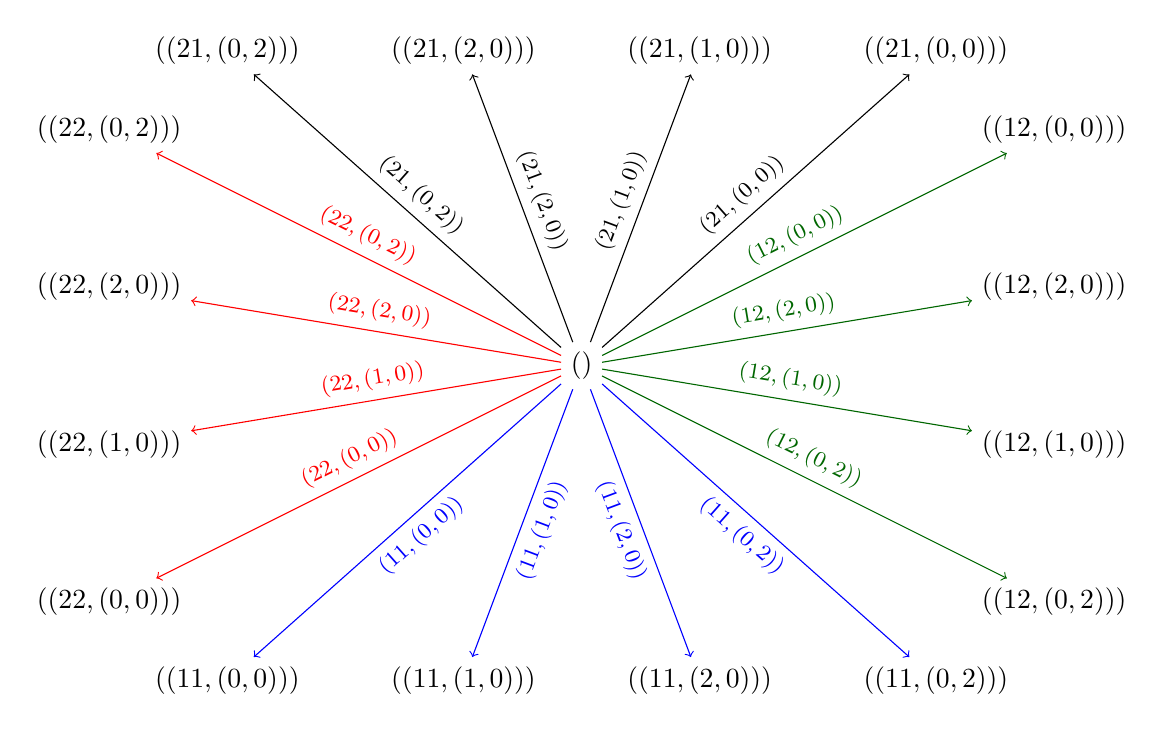
\begin{tikzpicture}
    \node (1) at (0,0) {$()$};
    
    \node (2) at (-4.5,-4) {$((11,(0,0)))$};
    \draw[->,blue] (1) -- (2) node[pos=0.5, below, sloped] {\footnotesize$(11,(0,0))$};
    \node (3) at (-1.5,-4) {$((11,(1,0)))$};
    \draw[->,blue] (1) -- (3) node[pos=0.5, below, sloped] {\footnotesize$(11,(1,0))$};
    \node (4) at (1.5,-4) {$((11,(2,0)))$};
    \draw[->,blue] (1) -- (4) node[pos=0.5, below, sloped] {\footnotesize$(11,(2,0))$};
    \node (14) at (4.5,-4) {$((11,(0,2)))$};
    \draw[->,blue] (1) -- (14) node[pos=0.5, below, sloped] {\footnotesize$(11,(0,2))$};
    
    \node (5) at (6,-3) {$((12,(0,2)))$};
    \draw[->,black!60!green] (1) -- (5) node[pos=0.5, above, sloped] {\footnotesize$(12,(0,2))$};
    \node (6) at (6,-1) {$((12,(1,0)))$};
    \draw[->,black!60!green] (1) -- (6) node[pos=0.5, above, sloped] {\footnotesize$(12,(1,0))$};
    \node (7) at (6,1) {$((12,(2,0)))$};
    \draw[->,black!60!green] (1) -- (7) node[pos=0.5, above, sloped] {\footnotesize$(12,(2,0))$};
    \node (15) at (6,3) {$((12,(0,0)))$};
    \draw[->,black!60!green] (1) -- (15) node[pos=0.5, above, sloped] {\footnotesize$(12,(0,0))$};
    

    \node (8) at (-4.5,4) {$((21,(0,2)))$};
    \draw[->] (1) -- (8) node[pos=0.5, above, sloped] {\footnotesize$(21,(0,2))$};
    \node (9) at (1.5,4) {$((21,(1,0)))$};
    \draw[->] (1) -- (9) node[pos=0.5, above, sloped] {\footnotesize$(21,(1,0))$};
    \node (10) at (-1.5,4) {$((21,(2,0)))$};
    \draw[->] (1) -- (10) node[pos=0.5, above, sloped] {\footnotesize$(21,(2,0))$};
    \node (16) at (4.5,4) {$((21,(0,0)))$};
    \draw[->] (1) -- (16) node[pos=0.5, above, sloped] {\footnotesize$(21,(0,0))$};

    \node (11) at (-6,-3) {$((22,(0,0)))$};
    \draw[->,red] (1) -- (11) node[pos=0.5, above, sloped] {\footnotesize$(22,(0,0))$};
    \node (12) at (-6,-1) {$((22,(1,0)))$};
    \draw[->,red] (1) -- (12) node[pos=0.5, above, sloped] {\footnotesize$(22,(1,0))$};
    \node (13) at (-6,1) {$((22,(2,0)))$};
    \draw[->,red] (1) -- (13) node[pos=0.5, above, sloped] {\footnotesize$(22,(2,0))$};
    \node (17) at (-6,3) {$((22,(0,2)))$};
    \draw[->,red] (1) -- (17) node[pos=0.5, above, sloped] {\footnotesize$(22,(0,2))$};


    \end{tikzpicture}
    \caption{Graf všech následníků počátečního stavu [2,2]-Mastermindu}
    \label{fignaslednicipocatecnihostavu22}
\end{figure}

Průběh [n,k]-Mastermindu s nějakým tajným kódem $v$ lze sledovat ve stromu [n,k]-Mastermindu. Nechť $A$ je stav a hráč zvolí další pokus $u$. Touto volbou hráč vybral část následníků, do kterých se stav hry může dostat. Jsou to právě následníci stavu $A$ vzhledem ke kódu $u$. Zadavatel ohodnotí kód $u$ vzhledem ke kódu $v$ ohodnocením $r$. Ohodnocením určí, který stav z následníků $A$ vzhledem ke kódu $u$ bude následovat. Hráč tedy může vybrat jako následující pokus ten, který bude mít nejvhodnější vrstvu následníků stavu $A$ (například podle množin kandidátů definovaných níže). Z těchto následníků ale neví, do kterého se hra dostane, protože nezná ohodnocení s tajným kódem. 


\subsubsection{Kandidát}
Pro každý stav lze nalézt množinu kódů, které by podle dostupných informací mohly být tajným kódem. 
% Jde o ty kódy, které mají s kódy ve stavu stejné ohodnocení jako příslušná ohodnocení ve stavu. 

\begin{definice}[Množina kandidátů]\label{kandidat}
  Pro počáteční stav definujeme \emph{množinu kandidátů} jako celý prostor kódů $H_{n,k}$. Nechť $A = \left((u_1, r_1), \dots, (u_j,r_j)\right), u_i \in H_{n,k}, r_i \in S_{n,k}$ je stav. \emph{Množinu kandidátů} stavu $A$ definujeme jako
  \[K = \{w \in H_{n,k} \mid s(w,u_i) = r_i,  i \in \{1,2,\dots ,j\} \}.\]
  Kód z této množiny nazveme \emph{kandidát}. 
  
  %Řekneme, že kód $u \in H_{n,k}$ je kandidát stavu $A$, pokud $s(u,u_i) = r_i \hspace{5px} \forall i \in \{1, \dots j\}$. 

  % Dále definujeme funkci $J$, která stavu přiřadí jeho množinu kandidátů.
  % \begin{align*}
  %     J \colon (H_{n,k} \times S)^+ &\to \mathbb{R} \\
  %       \left((u_1, r_1), (u_2,r_2), \dots, (u_j,r_j)\right) &\mapsto \{u \in H_{n,k} \mid s(u,u_i) = r_i \hspace{5px} \forall i \in \{1, \dots j\} \} 
  % \end{align*}
\end{definice}
Velikost a struktura množiny kandidátů určuje, jak blízko jsme uhodnutí tajného kódu.
% Množina kandidátů dává intuici za tím, jak blízko jsme uhádnutí tajného kódu. V případě, že množina kandidátů je jednoprvková, tak nám je znám tajný kód. Pokud je množina kandidátů veliká, nejspíš ještě budeme k rozlišení tajného kódu potřebovat více pokusů.
\begin{definice}[Potomek množiny]\label{defpotomekmnoziny}
  % Uvažujme [n,k]-Mastermind s nějakým tajným kódem $v\in H_{n,k}$. Nechť $S$ je množina všech ohodnocení v $H_{n,k}$. 
  Nechť $K \subseteq H_{n,k}$ je množina kódů, $u \in H_{n,k}$ je kód a $r \in S_{n,k}$ je ohodnocení. \emph{Potomka množiny $K$, vzhledem ke kódu $u$ a ohodnocení $r$} definujeme jako množinu 
  \[K_{u,r} = \{w \in K \mid s(w,u) = r\}.\] 
\end{definice}
\begin{pozn}
    \emph{Potomkem $K$, vzhledem ke kódu $u$} nazýváme množinu $K_{u,r}$ pro nějaké $r \in S_{n,k}$. \emph{Potomkem $K$} nazýváme množinu $K_{u,r}$ pro nějaké $u\in H_{n,k}$ a $r \in S_{n,k}$. 
\end{pozn}
Z definice plyne
\[\bigcup_{r\in S_{n,k}} K_{u,r} \subseteq K.\] Zároveň žádný kód $w \in K$ nemůže mít s kódem $u$ dvě různá ohodnocení, a tedy sjednocení je disjunktní. Navíc pro každý kód $w \in K$ platí, že $w \in K_{u, s(w,u)}$, a tedy platí následující lemma.

\begin{lemma}[Vztah množiny s jejími potomky]\label{lemmadisjunktnipotomci}
    % Nechť $S_{n,k}$ je množina všech ohodnocení kódů v $H_{n,k}$. 
    Pro každou množinu $K \subseteq H_{n,k}$ a kód $u \in H_{n,k}$ platí
    \[K = \bigsqcup_{r\in S_{n,k}} K_{u,r},\]
    tedy množina kódů je disjunktním sjednocením potomků vzhledem k určitému kódu.
\end{lemma}


% \begin{dukaz}
%     Dokážeme obě inkluze. Z definice $K_{u,r}$ platí 
%     \[\bigsqcup_{r\in S} K_{u,r} \subseteq K.\] 
%     Nechť $u \in H_{n,k}$. Potom pro každý kód $w \in K$ platí, že $w \in K_{u, s(u,w)}$ a tedy 
%     \[K \subseteq \bigsqcup_{r\in S} K_{u,r}.\] 
%     Zároveň žádný kód $w \in K$ nemůže mít s kódem $u$ dvě různá ohodnocení, a tedy sjednocení je disjunktní. 
% \end{dukaz}

% \begin{definice}[Graf \text{[n,k]-Mastermindu}]
%   Uvažujeme množinu vrcholů $\mathcal{V} = \mathcal{P}(H_{n,k})$ a množinu orientovaných hran $\mathcal{E}$ mezi vrcholy a jejich potomky. 
%   Cestu definujeme jako posloupnost navazujících hran. 
%   Definujeme $V \subseteq \mathcal{V}$ jako množinu vrcholů, do kterých vede cesta z vrcholu $H_{n,k}$. Graf [n,k]-Mastermindu definujeme jako indukovaný podgraf grafu $(\mathcal{V}, \mathcal{E})$ množinou $V$. Hranu $(K, K_{u,r})$ budeme značit jako hranu $(u,r)$ z vrcholu $K$.
% \end{definice}
\begin{lemma}[Vztah následníků a potomků]\label{lemmavztahnaslednikuapotomku}
    Uvažujme prostor kódů $H_{n,k}$. Nechť $A = \left((u_1, r_1), \dots, (u_j,r_j)\right)$ je stav a $K$ množina jeho kandidátů. Potom pro všechny kódy $u\in H_{n,k}$ a ohodnocení $r \in S_{n,k}$ platí, že $K_{u,r}$ je množina kandidátů stavu $A_{u,r}$.
    % stavu $A = \left((u_1, r_1), \dots, (u_j,r_j)\right)$, 
\end{lemma}
\begin{dukaz}
    Rozepíšeme z definic. 
    $K_{u,r} = \{w \in K \mid s(u,w) = r\}$ a $K = \{w \in H_{n,k} \mid s(u_i,w) = r_i,  i \in \{1,2,\dots ,j\} \}$. Tedy celkem 
    $K_{u,r}$ je množina kódů $w \in H_{n,k}$, pro které platí $s(u_i,w) = r_i$ pro $i \in \{1,2,\dots ,j\}$ a zároveň $s(u,w) = r$.
    Navíc platí, že $A_{u,r} = \left((u_1, r_1), \dots, (u_j,r_j), (u,r)\right)$. Lemma plyne z definice množiny kandidátů.
\end{dukaz}
Z lemmatu plyne, že potomci $K$ vzhledem ke kódu $u$ určují množiny kandidátů možných následující stavů v případě, kdy zvolíme kód $u$ jako další pokus. Množiny a jejich vztah s potomky zapíšeme do grafu. 

% \begin{definice}[Orientovaný multigraf]
%     \emph{Orientovaný multigraf} definujeme jako dvojici $G = (V,E)$. $V$ je množina vrcholů. $E \subseteq V \times V \times Q$ je množina hran s obarveními z množiny $Q$. Řekneme, že z vrcholu $K_1 \in V$ do vrcholu $K_2 \in V$ vede hrana obarvená $q \in Q$, pokud $(K_1, K_2, q) \in E$. Navíc $E$ je taková, že z libovolného vrcholu nevedou dvě různé hrany se stejným obarvením.
% \end{definice}
% \begin{pozn}
%     Orientovaný multigraf povoluje více hran mezi stejnými vrcholy, které se ale liší v obarvení. Hrana je navíc jednoznačně určená počátečním vrcholem a obarvením. Kořen je stejně jako v orientovaném grafu vrchol, do kterého nevede žádná hrana. 
% \end{pozn}
\begin{definice}[Multigraf prostoru kódů]
  Nechť $n, k\in \mathbb{N}$, $u\in H_{n,k}$ je kód a $r\in S_{n,k}$ je ohodnocení. \emph{Multigraf prostoru kódů} definujeme jako orientovaný graf $G_{n,k} = (\mathcal{V}, \mathcal{E})$. $\mathcal{V} = \mathcal{P}(H_{n,k})$ je množina vrcholů. $\mathcal{E} \subseteq \mathcal{V} \times \mathcal{V} \times (H_{n,k}\times S_{n,k})$ je množina hran s obarveními, pro kterou platí, že z vrcholu $K_1$ do vrcholu $K_2$ vede hrana obarvená $(u,r)$ právě tehdy, když $K_2$ je potomek $K_1$ vzhledem ke kódu $u$ a ohodnocení $r$. 
  % Každá hrana je jednoznačně určená počátečním vrcholem a obarvením $(u,r)$. 
  % kde každá hraná má přiřazené obarvení $r\in S_{n,k}$. 
\end{definice}
% Hrany v multigrafu jsou obarvené 


\begin{definice}[Multigraf {[n,k]-Mastermindu}]
  \emph{Multigraf [n,k]-Mastermindu} definujeme jako podgraf grafu $G_{n,k}$ indukovaný množinou vrcholů, do kterých vede nějaká orientovaná cesta z vrcholu $H_{n,k}$. 
  % Značíme ho $G_{n,k}^*$.
  
  %a množinu orientovaných hran $\mathcal{E}$ mezi vrcholy a jejich potomky. 
  %Cestu definujeme jako posloupnost navazujících hran. 
  %Definujeme $V \subset \mathcal{V}$ jako množinu vrcholů, do kterých vede cesta z vrcholu $H_{n,k}$. Graf [n,k]-Mastermindu definujeme jako indukovaný podgraf grafu $(\mathcal{V}, \mathcal{E})$ množinou $V$. Hranu $(K, K_{u,r})$ budeme značit jako hranu $(u,r)$ z vrcholu $K$.
\end{definice}
Z lemmatu \ref{lemmavztahnaslednikuapotomku} o vztahu následníků a potomků plyne, že vrcholy multigrafu [n,k]-Mastermindu jsou právě ty množiny, které odpovídají množinám kandidátů nějakého stavu. Mezi dvěma vrcholy může vést více hran, jak je vidět z multigrafu [1,2]-Mastermindu (viz obrázek \ref{fig-multigraf-12}).
% na obrázku \ref{figpotomciH22}, který zobrazuje neprázdné potomky $H_{2,2}$ vzhledem ke všem kódům a ohodnocením. 


\begin{figure}[h!]
    \centering
    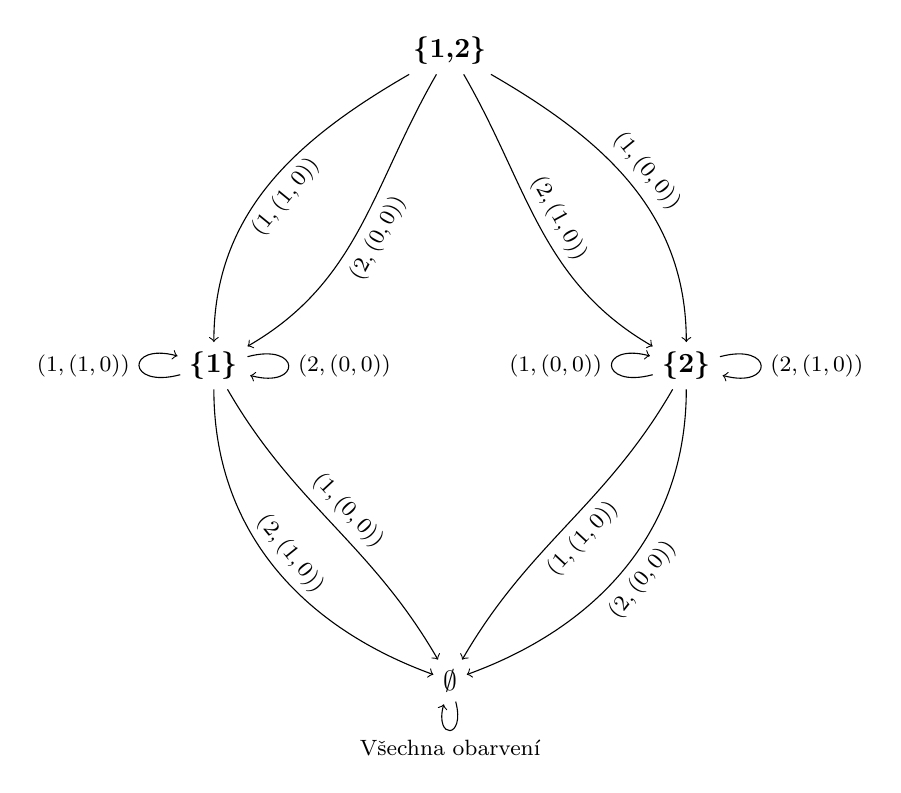
\begin{tikzpicture}
    \node (1) at (0,0) {\textbf{\{1,2\}}};
    \node (2) at (-3,-4) {\textbf{\{1\}}};
    \draw[->] (1) to[out=-150, in=90]  node[midway, below, sloped] {\footnotesize$(1,(1,0))$} (2);
    \draw[->] (1) to[out=-120, in=30] node[pos=0.5, below, sloped] {\footnotesize$(2,(0,0))$} (2);

    
    \node (3) at (3,-4) {\textbf{\{2\}}};
    \draw[->] (1) to[out=-30, in=90] node[pos=0.5, above, sloped] {\footnotesize$(1,(0,0))$} (3) ;
    \draw[->] (1) to[out=-60, in=150] node[pos=0.5, above, sloped] {\footnotesize$(2,(1,0))$} (3);

    \node (4) at (0,-8) {\textbf{$\emptyset$}};
    \draw[->] (2) to[out=-60, in=120] node[pos=0.5, above, sloped] {\footnotesize$(1,(0,0))$} (4);
    \draw[->] (2) to[out=-90, in=160] node[pos=0.5, above, sloped] {\footnotesize$(2,(1,0))$} (4);
    \draw[->] (3) to[out=-120, in=60]  node[midway, below, sloped] {\footnotesize$(1,(1,0))$} (4);
    \draw[->] (3) to[out=-90, in=20] node[pos=0.5, below, sloped] {\footnotesize$(2,(0,0))$} (4);
    \path[->] (2) edge [loop left] node {\footnotesize$(1,(1,0))$} ()
              (2) edge [loop right] node {\footnotesize$(2,(0,0))$} ()
              (3) edge [loop left] node {\footnotesize$(1,(0,0))$} ()
              (3) edge [loop right] node {\footnotesize$(2,(1,0))$} ()
              (4) edge [loop below] node {\footnotesize Všechna obarvení} ();
              %$\{1,2\} \times \{(1,0), (0,0)\}$
    \end{tikzpicture}
    \caption{Multigraf [1,2]-Mastermindu.}
    \label{fig-multigraf-12}
\end{figure}

Nyní ukážeme nějaké vlastnosti multigrafu [n,k]-Mastermindu, které pomohou ukázat jeho vztah se stromem [n,k]-Mastermindu. Název následující vlastnosti grafu byl převzat z různých publikací.
% zdroj - wikipedie, https://en.wikipedia.org/wiki/Directed_acyclic_graph
\begin{definice}[Orientovaně acyklický graf]
    Řekneme, že orientovaný graf je orientovaně acyklický, pokud neobsahuje žádný nekonstantní orientovaný cyklus.
\end{definice}
\begin{pozn}
    Tato vlastnost tedy povoluje hrany z vrcholu do sebe samotného. Ve chvíli, kdy ale hrana opustí vrchol, už se do něj po orientovaných hranách nelze vrátit. To připomíná vlastnost kořenového stromu až na existenci neorientovaných cyklů.
\end{pozn}

\begin{lemma}
    Multigraf [n,k]-Mastermindu je orientovaně acyklický. 
\end{lemma}
\begin{dukaz}
    Nechť existuje nějaký nekonstantní orientovaný cyklus. Potom existuje vrchol $K_1$, ze kterého cyklus vede a vrchol $K_2 \neq K_1$, přes který cyklus vede. Potom díky opakovanému použití lemmatu \ref{lemmadisjunktnipotomci} (přechod od vrcholu k neidentickým potomkům) platí $K_1 \subset K_2 \subset K_1$, což je spor. 
    % Potom existují vrcholy $K_1 \neq K_2$ multigrafu [n,k]-Mastermindu, přes které 
    % Pokud existuje nějaká cesta začínající i končící v $K_1$ vedoucí přes vrchol $K_2$, tak potom díky lemmatu \ref{lemmadisjunktnipotomci} platí $K_1 \subset K_2 \subset K_1$, což je spor. Tedy neexistuje žádná nekonstantní cesta začínající i končící ve stejném vrcholu.
\end{dukaz}
Touto vlastností chceme poukázat na vývoj stavu hry v případě hry Mastermind a zmenšování množiny kandidátů v dalších kolech. 

\begin{lemma}\label{lemmakandidatipocstavu}
    Množina kandidátů stavu $A$ je $H_{n,k}$ právě tehdy, když stav $A$ je počáteční.
\end{lemma}
\begin{dukaz}
    Množina kandidátů počátečního stavu je z definice celý prostor kódů. Stačí tedy dokázat implikaci \uv{\Rightarrow}. Nechť pro spor $A$ není počáteční stav. Označíme $K$ množinu jeho kandidátů. Bez újmy na obecnosti předpokládáme, že stav $A$ je složen právě z jednoho kódu s ohodnocením. Nechť $A = ((u, (b,w)))$. Pokud $(b,w) = (n,0)$, potom $K = \{u\}$. Pokud $(b,w) \neq (n,0)$, potom $u \notin K$. Tedy množina kandidátů stavu $A$ není $H_{n,k}$, což je spor. 
\end{dukaz}

Z lemmat plyne fakt, že multigraf [n,k]-Mastermindu má kořen, kterým je celý prostor kódů. Ve spojení s neexistencí nekonstantních orientovaných cyklů dostáváme podobnost multigrafu [n,k]-Mastermindu s kořenovým stromem [n,k]-Mastermindu. Tento vztah popíšeme formálně pomocí takzvaného rozvinutí.
% multigraf je "directed acyclic graph"
\begin{definice}[Rozvinutí grafu]
    \emph{Rozvinutí orientovaně acyklického grafu $G = (\mathcal{V}, \mathcal{E})$ s jedním kořenem} definujeme jako orientovaný graf $T = (V, E)$.
    % , kde $V$ je množina vrcholů a $E$ množina hran definované následovně.
    
    Množina vrcholů $V$ je množina cest z kořene grafu $G$, které jsou reprezentovány obarvením hran. Vrchol $A \in V$ je obarven vrcholem $K \in \mathcal{V}$, do kterého z kořene vede cesta $A$. 
    
    Pro množinu hran $E$ platí, že z vrcholu $A \in V$ do vrcholu $B \in V$ vede hrana právě tehdy, když cesta $B$ vznikne z cesty $A$ prodloužením o jednu hranu. Tato hrana je obarvená poslední hranou cesty $B$. 
\end{definice}
% Graf na obrázku \ref{fignaslednicipocatecnihostavu22} (výše) je rozvinutím multigrafu potomků $H_{2,2}$ na obrázku \ref{figpotomciH22}.

% \begin{figure}[h!]
%     \centering
%     \begin{tikzpicture}
%     \node (1) at (0,0) {\{11,12,21,22\}};
%     \node (4) at (-5,0) {\{11\}};
%     \draw[->] (1) to[out=165, in=30]  node[midway, below, sloped] {\footnotesize$(11,(2,0))$} (4);
%     \draw[->] (1) to[out=-165, in=-30] node[pos=0.5, below, sloped] {\footnotesize$(22,(0,0))$} (4);
%     \node (7) at (-3,4) {\{12\}};
%     \draw[->] (1) to[out=150, in=-90] node[pos=0.5, above, sloped] {\footnotesize$(12,(2,0))$} (7) ;
%     \draw[->] (1) to[out=120, in=-30] node[pos=0.5, above, sloped] {\footnotesize$(12,(2,0))$} (7);
%     \node (5) at (3,4) {\{21\}};
%     \draw[->] (1) to[out=90, in=-150] node[pos=0.5, above, sloped] {\footnotesize$(12,(0,2))$} (5);
%     \draw[->] (1) to[out=60, in=-90] node[pos=0.5, above, sloped] {\footnotesize$(21,(2,0))$} (5);
%     \node (2) at (5,0) {\{22\}};
%     \draw[->] (1) to[out=15, in=150] node[midway, above, sloped] {\footnotesize$(11,(0,0))$} (2);
%     \draw[->] (1) to[out=-15, in=-150] node[midway, above, sloped] {\footnotesize$(22,(2,0))$} (2);
%     \node (6) at (3,-4) {\{11, 22\}};
%     \draw[->] (1) to[out=-30, in=90] node[pos=0.5, above, sloped] {\footnotesize$(12,(1,0))$} (6);
%     \draw[->] (1) to[out=-60, in=150] node[pos=0.5, above, sloped] {\footnotesize$(21,(1,0))$} (6);
%     \node (3) at (-3,-4) {\{12, 21\}};
%     \draw[->] (1) to[out=-120, in=90] node[midway, below, sloped] {\footnotesize$(11,(1,0))$} (3);
%     \draw[->] (1) to[out=-90, in=30] node[midway, below, sloped] {\footnotesize$(22,(1,0))$} (3);
%     \end{tikzpicture}
%     \caption{Multigraf všech neprázdných potomků $H_{2,2}$}
%     \label{figpotomciH22}
% \end{figure}
% V případě multigrafu [n,k]-Mastermindu je obarvením vrcholu $A$ v rozvinutí množina kandidátů stavu $A$. 


\begin{veta}
    Strom [n,k]-Mastermindu je rozvinutím multigrafu [n,k]-Mastermindu.
\end{veta}
\begin{dukaz}
    Obarvení hran v multigrafu [n,k]-Mastermindu odpovídá kolům. Cesta z kořene reprezentovaná obarvením hran tedy přesně odpovídá nějakému stavu. Hrany mezi vrcholy rozvinutí a vrcholy stromu [n,k]-Mastermindu mají opět obdobný předpis. Z každého stavu ve stromě [n,k]-Mastermindu vedou hrany obarvené všemi kombinacemi kódů a ohodnocení. Obdobně každá cesta v multigrafu [n,k]-Mastermindu lze prodloužit hranou obarvenou libovolným kódem s ohodnocením. Prázdná cesta také odpovídá prázdnému stavu. Grafy jsou tedy identické. 
    
    % vrcholu, do kterého vede cesta $A$ v multigrafu [n,k]-Mastermindu začínající ve vrcholu $H_{n,k}$. 

     % chceme předpoklad, že hrana je jednoznačně určená počátečním vrcholem a obarvením, chtělo by to zmínit při konstrukci multigrafu, nebo při definici/označení cest v multigrafu. 

     % Nechť $A$ je vrchol ve stromu [n,k]-Mastermindu, potom $A$ značí i nějakou cestu v multigrafu. Z tohoto vrcholu vedou všechny možné hrany stejně tak jako z rozvinutí multigrafu [n,k]-Mastermindu. 

     % Z každého stavu vedou hrany obarvené všemi kódy s ohodnoceními. To samé platí pro vrcholy na multigrafu. 
\end{dukaz}
% Multigraf [n,k]-Mastermindu s umožňuje interpretovat hru bez znalosti 
Pro každý stav $A$ navíc díky lemmatu \ref{lemmavztahnaslednikuapotomku} platí, že jeho množina kandidátů je rovna obarvení ekvivalentního vrcholu v rozvinutí multigrafu [n,k]-Mastermindu. Pomocí multigrafu [n,k]-Mastermindu tedy lze určit množiny kandidátů všech stavů. Zadaný multigraf tedy umožňuje popsat množiny kandidátů bez znalosti ohodnocení. Možnost popisu hry pouze pomocí multigrafu krátce rozvedeme po následující sekci. 

% Bonus:
% \begin{definice}[Částečné uspořádání stavů??]
%     Definujeme částečné uspořádání stavů následovně. Množina stavů $\mathcal{A}$. Definujeme relaci $R \in \mathcal{A} \times \mathcal{A}$. 
%     Stav $A \in \mathcal{A}, B \in \mathcal{A}$. $(A,B) \in R$ pokud $A \subseteq B$, značíme $A \sim B$. Tato relace je částečné uspořádání, protože je tranzitivní
%     $A \subseteq B$ a $B\subseteq C$, potom $A \subseteq C$,
%     reflexivní $A \subseteq A$ a antisymetrická $A \subseteq B$ a $B\subseteq A$ implikuje $A = B$. 

%     Třídy ekvivalence - podle množiny kandidátů. Hrana vede z jedné třídy do druhé, pokud něco, nevím přesně jak to určit, 
% \end{definice}

% Pomocí toho lze definovat stavy, které odpovídají konci hry a případně prázdné stavy obarvené prázdnou množinou, do kterých se hra nikdy nedostane. 

% Multigraf tedy umožňuje popis hry bez nutnosti definování množiny kandidátů.

% Pokud bychom o použité hře nevěděli nic, ale měli bychom zadaný multigraf množin zbývajících možností, mohli bychom určit stavy, pro které je množina kandidátů jednoprvková, a tedy 

% Multigraf tedy popisuje vlastnosti všech stavů 

% Multigraf [n,k]-Mastermindu 

% Díky Lemmatu \ref{lemmavztahnaslednikuapotomku} můžeme popsat vztah mezi stromem a grafem [n,k]-Mastermindu. Nějaký vrchol $K$ grafu je množina kandidátů všech stavů, které odpovídají cestám z $H_{n,k}$ do tohoto vrcholu. 

% \begin{tvrz}[Vztah multigrafu a stromu \text{[n,k]-Mastermindu}]\label{tvrzenimultigrafastrom}
%     Nechť $A = \left((u_1, r_1), (u_2,r_2), \dots, (u_j,r_j)\right)$ je stav. a $K_1$ je jeho množina kandidátů. Nechť $K_2$ odpovídá vrcholu na konci cesty $A$ z $H_{n,k}$ multigrafem [n,k]-Mastermindu. Potom $K_1 = K_2$.  
% \end{tvrz}
% \begin{dukaz}
%     Postupujeme indukcí podle délky stavu. Nechť délka stavu je $1$, tvrzení platí díky lemmatu \ref{lemmavztahnaslednikuapotomku}. Nechť tvrzení platí pro $j\in \mathbb{N}, j\geq 2$. Potom $A = B_{u_{j+1}, r_{j+1}}$ pro nějaký stav $B$, kde množinu kandidátů $B$ označíme $K$. Potom $K$ je konec cesty $B$ z $H_{n,k}$ multigrafem [n,k]-Mastermindu z indukčního předpokladu. Potom z lemmatu \ref{lemmavztahnaslednikuapotomku} platí, že $K_{u_j, r_j}$, která je koncem cesty $A$ z $H_{n,k}$, je množina kandidátů stavu $A$. 
% \end{dukaz}


 


%%%%%%%%%%%%%%%%%%%%%%%%%%%%%%%%%%%%%%%%%%%%%%%%%%%%%%%%%%%%%%%%%%%%%%%%%%%%%


\subsubsection{Strom algoritmu}
V této sekci definujeme takzvaný strom algoritmu, který zobrazuje průběh hry [n,k]-Mastermind pro všechny tajné kódy v případě pevně zvoleného algoritmu. 

\begin{definice}[Prázdný a koncový stav]\label{kandidat}
  % Nechť $A = \left((u_1, r_1), \dots, (u_j,r_j)\right), u_i \in H_{n,k}, r_i \in S_{n,k}$ je stav. 
  Řekneme, že stav $A$ je \emph{prázdný}, pokud je množina kandidátů tohoto stavu prázdná. Řekneme, že stav $A$ je \emph{koncový}, pokud je neprázdný a poslední kolo je rovno $(u,(n,0))$ pro nějaký kód $u$.
\end{definice}

Prázdný stav nemůže odpovídat průběhu hry Mastermind, protože v tu chvíli žádný kód nemůže být tajným kódem. V reálné hře by ho šlo dosáhnout pouze při chybě v ohodnocení pokusu. Koncový stav odpovídá konci hry, kdy se pokus shoduje s tajným kódem. Množina jeho kandidátů v tu chvíli obsahuje právě tajný kód. 


\begin{definice}[Strom algoritmu]
  Řekneme, že konečný souvislý podgraf $T$ stromu [n,k]-Mastermindu je \emph{strom algoritmu}, pokud splňuje následující podmínky.
  % Strom algoritmu definujeme jako souvislý podgraf stromu [n,k]-Mastermindu, který splňuje následující podmínky.
  \begin{enumerate}
      \item Neobsahuje prázdné stavy.
      \item Hrany vedoucí z každého vrcholu grafu $T$ jsou obarveny nejvýše jedním kódem. Pro stav $A$ tento kód označíme $u_A$.
      \item Pro každý kód $w \in H_{n,k}$ má graf $T$ právě jeden koncový stav s posledním členem $(w, (n,0))$, který je navíc listem v $T$.
  \end{enumerate}
\end{definice}

\begin{tvrz}\label{tvrzkorenstromualg}
    Strom algoritmu má kořen a je jím počáteční stav. 
\end{tvrz}
\begin{dukaz}
    Z tvrzení \ref{tvrzeni-podgraf-korenoveho-stromu} plyne, že strom algoritmu je kořenový strom. Označíme $K$ množinu kandidátů jeho kořene. Chceme ukázat, že $K = H_{n,k}$.
    % Strom algoritmu neobsahuje žádné orientované cykly (cesty se začátkem i koncem ve stejném vrcholu) díky definici hran.
    % ve stromě [n,k]-Mastermindu. 
    % Zároveň do každého stavu (kromě počátečního) vede právě jedna hrana a díky souvislosti tedy strom algoritmu obsahuje nějaký kořen. Označíme $K$ množinu jeho kandidátů.
    Využijeme lemmatu \ref{lemmavztahnaslednikuapotomku} a lemmatu \ref{lemmadisjunktnipotomci} o disjunktním sjednocení potomků množin kandidátů. Díky podmínce $2$ z definice stromu algoritmu jsou množiny kandidátů všech stavů ve stromu algoritmu podmnožinami $K$. Pokud $K \neq H_{n,k}$, existoval by kód $u \in H_{n,k} \setminus K$. Pokud by potom strom algoritmu obsahoval stav s kolem $(u, (n,0))$, tento stav by byl prázdný. Nemohl by tedy pro tento kód existovat koncový stav. Množina kandidátů kořene je tedy rovna $H_{n,k}$. Z lemmatu \ref{lemmakandidatipocstavu} plyne, že kořenem je právě počáteční stav. 
\end{dukaz}

\begin{definice}
    Řekneme, že stav $B$ je \emph{prodloužením stavu} $A$, značíme $A \leq B$, pokud existuje orientovaná cesta ve stromu [n,k]-Mastermindu ze stavu $A$ do stavu $B$. 
\end{definice}


\begin{lemma}\label{lemmaprunikacestastromalg}
    Nechť $T = (V,E)$ je strom algoritmu a $A_1, A_2 \in V$ jsou neprázdné stavy s množinami kandidátů $K_1, K_2 \subseteq H_{n,k}$. Potom $A_1 \leq A_2$ nebo $A_2 \leq A_1$ právě tehdy, když průnik $K_1$ a $K_2$ je neprázdný.
    % Uvažujeme cesty v $T$ z počátečního stavu do obou stavů. Potom platí, že cesta do $A_2$ je prodloužením cesty do $A_1$ nebo je s ní shodná, značíme $A_1 \leq A_2$, právě tehdy, když průnik $K_1$ a $K_2$ je neprázdný. 
\end{lemma}
\begin{dukaz}
    Dokážeme obě implikace. Nechť napřed jedna cesta je prodloužením druhé, například $A_1 \leq A_2$. Potom z opakovaného použití lemmat \ref{lemmavztahnaslednikuapotomku} a \ref{lemmadisjunktnipotomci} plyne, že $K_2 \subseteq K_1$. Obě množiny jsou neprázdné, a tedy jejich průnik je neprázdný. 

    Druhou implikaci dokážeme indukcí podle součtu délek cest z počátku do stavů $A_1$ a $A_2$. Délky označíme $d_1$ a $d_2$. Nechť $d_1 + d_2 = 1$ a průnik $K_1$ a $K_2$ je neprázdný. Potom jeden stav je počáteční a druhý je jeho následník, a tedy jedna cesta je prodloužením druhé.
    % Tedy z lemmatu \ref{lemmadisjunktnipotomci} platí, že jedna množina je podmnožinou druhé, jejich průnik je tedy neprázdný. .

    % Nechť $d = 2$. Potom buď délka obou cest je stejná, a tedy jsou oba stavy následníky počátečního. Tedy z lemmatu \ref{lemmadisjunktnipotomci} je jedna cesta prodloužením druhé (v tomto případě shodná cesta) právě tehdy, když je průnik množin kandidátů neprázdný.

    Nechť tvrzení platí pro $m \in \mathbb{N}$ a $d_1 + d_2 = m+1$ a například $d_2 \geq d_1$. Označíme $B \in V$ stav, ze kterého vede do stavu $A_2$ hrana, $K$ množinu jeho kandidátů a $d = d_2-1$ délku cesty z počátku do $B$. Nechť průnik $K_1$ a $K_2$ je neprázdný. Z lemmatu \ref{lemmadisjunktnipotomci} plyne $K_2 \subseteq K$, a tedy průnik $K$ a $K_1$ je neprázdný. Pokud $d_2 > d_1$, tak z indukčního předpokladu a délek cest plyne, že $A_1 \leq B$. Navíc $B\leq A_2$, a tedy $A_1 \leq A_2$. Pokud $d_2 = d_1$, tak z indukčního předpokladu a délek cest plyne $B \leq A_1$. Navíc $d_1 = d+1$, a tedy $A_1$ je stejně jako $A_2$ následník $B$. Z podmínky $2$ v definici stromu algoritmu a lemmatu \ref{lemmadisjunktnipotomci} plyne, že $A_1 = A_2$, a tedy $A_1 \leq A_2$. 
\end{dukaz}


\begin{tvrz}\label{tvrzvsichninaslednici}
    Z každého nekoncového vrcholu $A$ stromu algoritmu vedou hrany do všech neprázdných následníků vzhledem k $u_A$.
\end{tvrz}
\begin{dukaz}
    Nechť existuje nekoncový stav $A$ ve stromu algoritmu $T = (V,E)$ s množinou kandidátů $K$, ze kterého nevede hrana do nějakého neprázdného následníka vzhledem k $u_A$. Tedy z lemmatu \ref{lemmadisjunktnipotomci} existuje nějaký kód $w \in K$, který nenáleží do žádné množiny kandidátů následníků $A$ v $T$. 

    Z definice stromu algoritmu ale existuje nějaký koncový stav $B$ s posledním členem $(w,(n,0))$, který má množinu kandidátu jednoprvkovou množinu $\{w\}$. Platí, že $K\cap \{w\} \neq \emptyset$, a tedy díky lemmatu \ref{lemmaprunikacestastromalg} $A \leq B$ nebo $B \leq A$. Protože koncový stav je listem, tak musí platit $A \leq B$. Tedy existuje posloupnost stavů, které leží na cestě z $A$ do $B$. Znovu díky lemmatu \ref{lemmaprunikacestastromalg} musí každá množina kandidátů těchto stavů obsahovat kód $w$. Konkrétně tedy nějaká množina kandidátů následníka $A$ v $T$ musí obsahovat $w$. Což je ale spor s předpokladem, že $w$ nenáleží do žádné množiny kandidátů následníků $A$ v $T$. Tedy z každého vrcholu $A$ stromu algoritmu vedou hrany do všech neprázdných následníků $A$ vzhledem k $u_A$. 
\end{dukaz}

% Nyní předpokládejme, že máme nějaký algoritmus výběru dalšího tahu a pro každý dosažitelný stav $A$ [n,k]-Mastermindu známe následující zahraný kód $u_A$. Potom lze sestavit takzvaný strom algoritmu, který zobrazuje pro každý stav $A$ potomky vzhledem k zahranému kódu $u_A$. 

% Prázdné stavy jsou vynechány, protože jsou v průběhu hry nedosažitelné. Potomky koncových stavů neuvažujeme, protože by to byly pokusy po konci hry. 
\begin{pozn}
    Uvažujme algoritmus $\mathcal{Z}$ který pro stav $A$ zahraje kód $u_A$ určený pro tento stav. Potom strom tohoto algoritmu lze sestavit rekurzivně, kdy napřed obsahuje pouze počáteční stav. Pro každý nekoncový stav $A$ ve stromu algoritmu přidáme do stromu všechny neprázdné následníky $A$ vzhledem k zahranému kódu $u_A$ a hrany, které je spojují se stavem $A$. 
    % Tento orientovaný graf nazýváme strom algoritmu $\mathcal{Z}$. 
    Pokud je algoritmus zvolen vhodně, tento orientovaný graf splňuje podmínky z definice, protože proces skončí až u koncových stavů a v každém kroku jsou všechny kódy z množiny kandidátů stavu $A$ obsaženy v množině kandidátů nějakého následníka.
\end{pozn}
 Strom algoritmu popisuje průběh hry pro všechny tajné kódy. Jednotlivá kola [n,k]-Mastermindu s tajným kódem $v\in H_{n,k}$ odpovídají hranám cesty z počátečního stavu do koncového stavu s posledním kolem $(v,(n,0))$. Příklad stromu algoritmu pro [2,2]-Mastermind ukazuje obrázek \ref{figprikladstromualgoritmu}. Stejný strom vytvoříme postupně v příkladu v další sekci a ukážeme, že to doopravdy je strom algoritmu. Ze stromu algoritmu lze vyčíst počty pokusů, které algoritmus potřebuje k nalezení tajných kódů. Jsou to délky cest od kořene k listům.

    %Platí, že pro nějaký kód $u$ jsou množiny kandidátů potomků $A$ vzhledem ke kódu $u$ disjunktní a sjednocením dávají množinu kandidátů stavu $A$. Všechny stavy, do kterých se dostaneme cestou z nějakého stavu $A$ za dodržení podmínky $1$ tedy mají kandidáty z množiny kandidátů stavu $A$. 


%\begin{pozn}
    %Stavy budeme také označovat množinou kandidátů pro tento stav. Množina kandidátů neurčuje jednoznačně stav (například prohozením prvků stavu bychom došli do stejné množiny kandidátů). Naopak stav jednoznačně určuje množinu kandidátů. 
%\end{pozn}

\begin{figure}[h!]
    \centering
    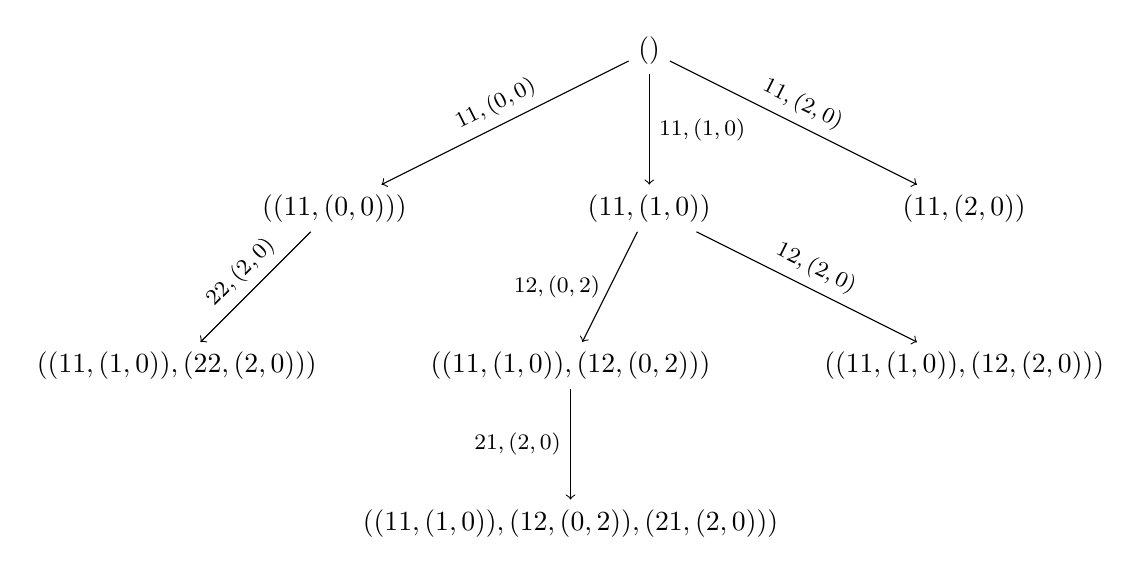
\begin{tikzpicture}
    \node (1) at (0,0) {$()$};
    \node (2) at (-4,-2) {$((11,(0,0)))$};
    \draw[->] (1) -- (2) node[pos=0.5, above, sloped] {\footnotesize{$11,(0,0)$}};
    \node (3) at (0,-2) {$(11,(1,0))$};
    \draw[->] (1) -- (3) node[pos=0.5, right] {\footnotesize{$11,(1,0)$}};
    \node (4) at (4,-2) {$(11,(2,0))$};
    \draw[->] (1) -- (4) node[pos=0.5, above, sloped] {\footnotesize{$11,(2,0)$}};
    \node (5) at (-1,-4) {$((11,(1,0)), (12,(0,2)))$};
    \draw[->] (3) -- (5) node[pos=0.5, left] {\footnotesize{$12,(0,2)$}};
    \node (6) at (4,-4) {$((11,(1,0)), (12,(2,0)))$};
    \draw[->] (3) -- (6) node[pos=0.5, above, sloped] {\footnotesize{$12,(2,0)$}};
    \node (7) at (-6,-4) {$((11,(1,0)), (22,(2,0)))$};
    \draw[->] (2) -- (7) node[pos=0.5, above,sloped] {\footnotesize{$22,(2,0)$}};
    \node (8) at (-1,-6) {$((11,(1,0)), (12,(0,2)), (21,(2,0)))$};
    \draw[->] (5) -- (8) node[pos=0.5, left] {\footnotesize{$21,(2,0)$}};
    \end{tikzpicture}
    \caption{Strom algoritmu pro [2,2]-Mastermind.}
\label{figprikladstromualgoritmu}
\end{figure}

\subsubsection{Zobecnění hledání optimálního algoritmu}
Hledání algoritmu s nejlepším průměrným nebo maximálním počtem pokusů lze převést na hledání stromu algoritmu, který bude mít maximální nebo průměrnou délku cesty od kořene do listu co nejmenší. Strom algoritmu lze navíc najít také jako podgraf rozvinutí multigrafu [n,k]-Mastermindu. Díky tomu lze popsat hledání algoritmů (stromů algoritmů) s nejlepšími výsledky pouze pomocí multigrafu [n,k]-Mastermindu. 

Obdobný postup by šel aplikovat na mnoho dalších her ve formě hádání tajného prvku pomocí pokládání otázek. Nechť máme nějakou množinu prvků $H$ a sadu otázek. Každému prvku přiřadíme pro každou otázku nějakou odpověď. Poté lze sestrojit orientovaný graf na množině podmnožin $H$, s hranami obarvenými otázkou a odpovědí. Pokud by z vrcholu $A$ do vrcholu $B$ vedla hrana $(u,r)$, množina $B$ by byla množina těch prvků z $A$, které mají na otázku $u$ odpověď $r$. 

Problém lze dále zobecnit na situaci, kdy o původním problému nic nevíme, ale máme zadaný nějaký orientovaný graf na množinách prvků. Pomocí rozvinutí a následného hledání stromu algoritmu by šlo nalézt optimální algoritmus, který nalezne libovolný prvek původní množiny na co nejmenší počet otázek. Koncový stav lze v tomto případě definovat jako situaci, kdy je obarvení vrcholu rozvinutého grafu rovno jednoprvkové množině. Prázdný stav lze interpretovat jako vrchol rozvinutí, který je obarven prázdnou množinou. 
% Zde se odkazujeme na možnost obarvení vrcholů při rozvinutí v poznámce \ref{poznobarvenivrcholurozvinuti} pod definicí rozvinutí.

% Ve chvíli, kdy bychom dostali multigraf vycházející z nějaké množiny prvků a sady otázek a odpovědí vyhovujících pro každý prvek množiny. Hrany by byly obarvené otázkou s odpovědí a množina prvků, do které by hrana vedla by byla právě množina prvků z původní množiny,

% \begin{definice}[Strom algoritmu \text{[n,k]-Mastermindu}]
%   Řekneme, že souvislý podgraf $T$ rozvinutí multigrafu [n,k]-Mastermindu je strom algoritmu, pokud splňuje následující podmínky.
%   % Strom algoritmu definujeme jako souvislý podgraf stromu [n,k]-Mastermindu, který splňuje následující podmínky.
%   \begin{enumerate}
%       \item Neobsahuje vrcholy obarvené prázdnou množinou.
%       \item Hrany vedoucí z každého vrcholu grafu $T$ jsou obarveny nejvýše jedním kódem. 
%       \item Pro každý kód $w \in H_{n,k}$ má graf $T$ právě jeden koncový stav s posledním členem $(w, (n,0))$, který je zároveň listem v grafu $T$.
%   \end{enumerate}
% \end{definice}


% Uvažujme nějaký algoritmus, který pro každý stav, do kterého se za použití algoritmu můžeme dostat, vybere deterministicky nějaký další pokus. Strom algoritmu lze sestrojit rekurzivně. Pro každý stav $A$ algoritmus nalezne další pokus $u_A$. Do stromu zakreslíme všechny neprázdné následníky stavu $A$ vzhledem k $u_A$.




\section{Obecný algoritmus}
Nyní přistoupíme k popisu skupiny deterministických algoritmů řešící hru [n,k]-Mastermind. V této práci popisujeme algoritmy, které pro libovolný stav $A$ vybírají další pokus podle množiny kandidátů stavu $A$. 
Pro dva různé stavy, které ale mají shodnou množinu kandidátů je problém nalezení dalšího kódu ekvivalentní. Předpokládáme totiž, že všechny kódy mohou být tajným kódem se stejnou pravděpodobností. 
Tento výběr popíšeme pomocí dvou funkcí, valuace a strategie. 


% Algoritmy popisujeme podle funkcí, které pro jakýkoliv stav naleznou další pokus. Nazýváme je, valuace a strategie. 

% Tyto funkce definujeme pro množiny kandidátů stavů. 

% Množiny kandidátů pro nás budou sloužit jako vnitřní stavy, pomocí kterých vybíráme další pokusy. Pro dva různé stavy, které ale mají shodnou množinu kandidátů je problém nalezení dalšího kódu ekvivalentní. Předpokládáme totiž, že všechny kódy mohou být tajným kódem se stejnou pravděpodobností. 



% Pro zjednodušení tyto funkce definujeme pro množiny kandidátů stavů. Pro dva různé stavy, které ale mají shodnou množinu kandidátů je problém nalezení dalšího kódu ekvivalentní. Předpokládáme totiž, že všechny kódy mohou být tajným kódem se stejnou pravděpodobností. Stejné množiny kandidátů pro dva různé stavy lze například dosáhnout prohozením prvků stavu. 

% Ve chvíli, kdy mají nějaké dva stavy stejnou množinu kandidátů, nezáleží na tom, jaké prvky stav obsahuje. Platí, že při následném zvolení stejných pokusů pro oba stavy dosáhneme stejného výsledku. Dojdeme ke stejnému konečnéme stavu.

% Pro dva různé stavy, které ale mají shodnou množinu kandidátů je problém nalezení dalšího kódu ekvivalentní. Předpokládáme totiž, že všechny kódy mohou být tajným kódem se stejnou pravděpodobností. Stejné množiny kandidátů pro dva různé stavy lze například dosáhnout prohozením prvků stavu. 


% K popisu výběru dalšího tahu algoritmy nebudou používat stav hry jako v definici \ref{defstav}. Místo toho vybírají další kód za pomocí množiny kandidátů tohoto stavu. 

% Našim cílem je totiž co nejlépe rozlišit, který kandidát je tajným kódem. Různé stavy které ale mají stejnou množinu kandidátů se v této informaci neliší. Proto výběr dalšího tahu lze vztáhnout pouze na množinu kandidátů aktuálního stavu. 



% U této definice si nejsem jistý, jak to smyslupně definovat. Vazba "která lz e vyjádřit pomocí potomků" se mi moc nelíbí - definovat valuaci a až potom jednokrokové valuace
\begin{definice}[Valuace]
    Nechť $K \subseteq H_{n,k}$ je množina kódů. Potom \emph{valuaci vzhledem k množině $K$} definujeme jako funkci $f_K(u) \colon H_{n,k} \to \mathbb{R}$.
\end{definice}


Valuace bude v algoritmech sloužit pro vyčíslení vhodnosti kódu $u$ jako dalšího pokusu pro stav s množinou kandidátů $K\subseteq H_{n,k}$. Tato hodnota bude obvykle záviset na potomcích $K$ vzhledem ke kódu $u$. Valuaci tedy lze interpretovat jako funkci, která nahlíží v multigrafu [n,k]-Mastermindu do následujících vrcholů.

% Valuace nám umožňuje ohodnotit kód podle toho, jak dobré jsou jeho následující stavy. Valuace by nemusela být omezená na následující vrstvu. Mohla by odkazovat na stavy o více než jednu hranu dál.

\begin{prikl}\label{prjednokrokfce}
    Funkce $f_K$ je příklad valuace, která kódu $u$ přiřadí maximální počet kódů potomka $K$ vzhledem ke kódu $u$.
    % jednokrokov8 funkce je taková, která kódu $u$ přiřadí hodnotu, která lze vyjádřit pomocí potomků $K$ vzhledem ke kódu $u$.
    \begin{align*}
        f_K \colon H_{n,k} &\to \mathbb{R} \\
        u &\mapsto \max_{r\in S} |K_{u,r}|
    \end{align*}
    % Pro $K = H_{2,2}$ z obrázku \ref{fig22prvnitah} má $f_{K}$ konstantní hodnotu $\frac{3}{2}$.
\end{prikl}
% množinu kandidátů na tajný kód


\begin{definice}[Strategie]
    Nechť $\mathcal{F} = \{f_K\colon H_{n,k} \to \mathbb{R} \mid K \subseteq H_{n,k}\}$ je prostor valuací. Potom řekneme, že zobrazení $F \colon \mathcal{F} \to \mathbb{R}$ je \emph{strategie}, pokud pro každou $f_K \in \mathcal{F}$ existuje $u\in H_{n,k}$ takové, že $F(f_K) = f_K(u)$.
\end{definice}
% Strategie určitým způsobem slouží k výběru následujícího kódu. 
%Zjednodušeně řečeno slouží k určení, 
Strategie určuje kritérium, podle kterého se vybírá další pokus. Algoritmy budou vybírat právě ty kódy, které mají valuaci rovnou hodnotě strategie pro aktuální množinu kandidátů. 

% v této práci bude určovat, zda chceme vybírat kódy s vyšší nebo nižší hodnotou valuace.
%Použití bude popsáno níže v popisu algoritmu \ref{alg-default}. 

\begin{prikl}\label{prstrategie}
    Následující funkce $F$ je strategie.
    \[F(f_K) =  \max_{u\in H_{n,k}} f_K(u)\]
    Funkce $F$ je dobře definovaná, protože maximum na konečné množině reálných čísel má vždy jednoznačně určenou hodnotu. Navíc existuje $u\in H_{n,k}$, pro který platí $f_K(u) = \max_{u\in H_{n,k}} f_K(u)$, a tedy $F$ je strategie.
\end{prikl}

\begin{definice}[Deterministický algoritmus]\label{defobecnyalg}
    \emph{Deterministický algoritmus řešící [n,k]-Mastermind s prostorem valuací $\mathcal{F}$ a strategií $F$} je funkce, která tajnému kódu $v$ přiřadí posloupnost zahraných kódů s ohodnoceními $\textsc{Solve}[n, k, \mathcal{F}, F](v)$, podle předpisu algoritmu \ref{alg-default}.
    
    % podle předpisu funkce \textsc{Solve} v algoritmu \ref{alg-default} jako
    % % definujeme jako algoritmus se zvoleným prostorem valuací $\mathcal{F}$ a zvolenou strategií $F$ popsaný pro vstupní tajný kód $v$ v algoritmu \ref{alg-default}. 
    % \begin{align*}
    %     \textsc{Solve}[n, k, \mathcal{F}, F] \colon H_{n,k} &\to \mathbb{N} \\
    %     v & \mapsto \textsc{Solve}[n, k, \mathcal{F}, F](v).
    % \end{align*}
    
    % které pro následující pokus vybírají kód podle zvolené valuace a strategie. Postup je znázorněn v algoritmu \ref{alg-default}.
    
\end{definice}
\begin{pozn}
    Důkaz správnosti algoritmu bude sestrojen pro konkrétní volby valuace a strategie v následující kapitole. 
\end{pozn}


% \subsection{Varianty algoritmů}





%Nechť \[P = \left((u_1, r_1), (u_2,r_2), \dots, (u_j,r_j)\right), u_i \in H_{n,k}, r_i \in \N _0 \times \N _0\] jsou tahy s ohodnocením a $K$ je konec cesty $P$ z vrcholu $H_{n,k}$. 

%Potom jednokrokové strategie volí další kód ten, který minimalizuje respektive maximalizuje funkci $f_K$. Pokud je těchto kódů více, zvolí kód, který je zároveň kandidát cesty $P$. Pokud výběr stále není jednoznačný, algoritmus zvolí lexikograficky nejnižší kód. 

\begin{algorithm}[h!]
\begin{algorithmic}[1]  % [1] způsobí, že číslujeme kroky algoritmu
\Function{Solve$[n, k, \mathcal{F}, F]$}{$v$}
    \State $K \gets H_{n,k}$ 
    \State $j \gets 0$
    \State $r_0 \gets (0,0)$
    \While {$r_j \neq (n,0)$} \hfill \mbox{(dokud hra není dohrána)}
        \State $j \gets j + 1$ 
	\State $U \gets \{u \in H_{n,k} \mid f_K(u) = F(f_K)\}$
        \If{$U \cap K \neq \emptyset$}
            \State $u_j \gets$ lexikograficky nejmenší $u \in U \cap K$
	\Else
		\State $u_j \gets$ lexikograficky nejmenší $u \in U$
	\EndIf
        \State $r_j \gets s(u_j, v)$ \hfill \mbox{(ohodnocení pokusu)}
        \State $K \gets K_{u_j,r_j}$
    \EndWhile
    \State \Return $((u_1,r_1),\dots,(u_j, r_j))$ \hfill \mbox{($j$ je počet pokusů a $u_j$ je tajný kód)}
\EndFunction
\end{algorithmic}
\caption{Deterministický algoritmus řešící [n,k]-Mastermind}
\label{alg-default}
\end{algorithm}

Písmenem $K$ značíme množinu kandidátů na tajný kód pro aktuální stav hry. Ta vždy odpovídá aktuálnímu stavu díky lemmatu \ref{lemmavztahnaslednikuapotomku} o vztahu mezi následníky stavů a potomky množin kandidátů. Tajný kód $v$ náleží do množiny kandidátů $K$ v každé iteraci, protože 
\[v \in K_{u_j, s(u_j,v)} = K_{u_j, r_j}.\]

Hra začíná s počátečním stavem, a tedy počáteční množina kandidátů v~algoritmu je $K = H_{n,k}$. Kód, který algoritmus zvolí jako j-tý pokus značíme $u_j$. Jeho ohodnocení vzhledem k tajnému kódu $v$ značíme $r_j$. Množina $U$ značí kódy, ve~kterých valuace $f_K$ nabývá nejlepší hodnotu danou strategií $F$. Z této množiny algoritmus vybírá další pokus $u_j$. Ve chvíli, kdy existuje kandidát v množině $U$ ($U\cap K \neq \emptyset$), algoritmus zvolí ten, který je lexikograficky nejmenší. V opačném případě algoritmus volí lexikograficky nejmenší kód z $U$. Množina $U$ nikdy nebude prázdná díky podmínce z definice strategie (valuace $f_K$ nabývá hodnotu strategie $F(f_K)$). 

% ================= šlo by přidat/změnit definici determ.alg. ================
Obecně tedy platí, že deterministický algoritmus s prostorem valuací $\mathcal{F}$ a~strategií $F$ je takový algoritmus, který pro stav $A$ s množinou kandidátů $K$ volí další pokus z množiny $U = \{u \in H_{n,k} \mid f_K(u) = F(f_K)\}$. Pokud $U \cap K \neq \emptyset$, volí lexikograficky nejmenší $u \in U \cap K$, jinak volí lexikograficky nejmenší $u \in U$. Tento postřeh využijeme k sestrojení stromu algoritmu pro konkrétní algoritmus.


% šlo by napsat pro dvojice funkce f, funkcionál F
%\begin{veta}[Správnost algoritmu \ref{alg-default}]
 %   Algoritmus \ref{alg-default}
%\end{veta}

% \begin{tvrz}[Počet ohodnocení]
% Nechť $n\in \mathbb{N}, k\in \mathbb{N}, k \geq 3$. Potom počet všech možných ohodnocení kódů v $H_{n,k}$ je $\frac{n^2 + 3n}{2}$.
% \end{tvrz}
% \begin{dukaz}
% Pro $b \leq n,\hspace{3px} b \neq n-1$ černých kolíčků existuje $n-b+1$ možností na počet bílých kolíčků podle tvrzení \ref{tvrzohodnoceni}. Pro $b = n-1$ existuje pouze jedno ohodnocení. Součtem přes počet černých kolíčků dostáváme následující počet možností ohodnocení.
%     \[|S| = (n+1) + n + (n-1)  + \dots + 3 + 1 + 1 \]
% Vzorcem pro součet aritmetické řady se dobereme k výsledku.
%     \[|S| = \frac{(n+1)(n+2)}{2} - 1 \]
%     \[|S| = \frac{n^2 + 3n}{2}\]
% \end{dukaz}

% \begin{tvrz}[Časová složitost algoritmu \ref{alg-default}]
%     Uvažujeme případ, kdy $F$ je minimizér/maximizér.
%     Algoritmus \ref{alg-default} má časovou složitost
%     % \[O( k^n O(f_K))\]
%     \[O \left( \sum_{j = 1}^z k^n \cdot m_j \cdot n^2 \cdot \frac{n^2 + 3n}{2}\right)\]
    
% \end{tvrz}
% \begin{dukaz}
%     $k^n$ je počet všech kódů, které musím projít, abych našel ten nejlepší, $m_j$ je maximální počet kandidátů v j-té iteraci, $z$ je maximální počet iterací algoritmu. $\frac{n^2 + 3n}{2}$ je počet všech ohodnocení, $n^2$ je časová složitost ohodnocení.

%     Potřebuji ještě limit na počet iterací $z$, horní odhad na $m_j$ a zjistit složitost nalezení průniku $U$ a $K$.
% \end{dukaz}
